\chapter{Code Listing}
As per request of the assignment, this chapter provides the reader with the
code listing. Due to the modular nature of Object-Oriented Programming, the
code cannot be provided as a single script. Therefore, the UML class diagram is
provided first to give an overview as to how the various code listings relate
to each other. Furthermore, due to the relatively large---as compared to a
typical engineering script---code-base only the critical bits of code have been
provided. For a full listing, the reader is invited to check out the GitHub
repository\footnote{\url{https://github.com/skilkis/numfoil}}.

\begin{figure}[H]
    \centering
    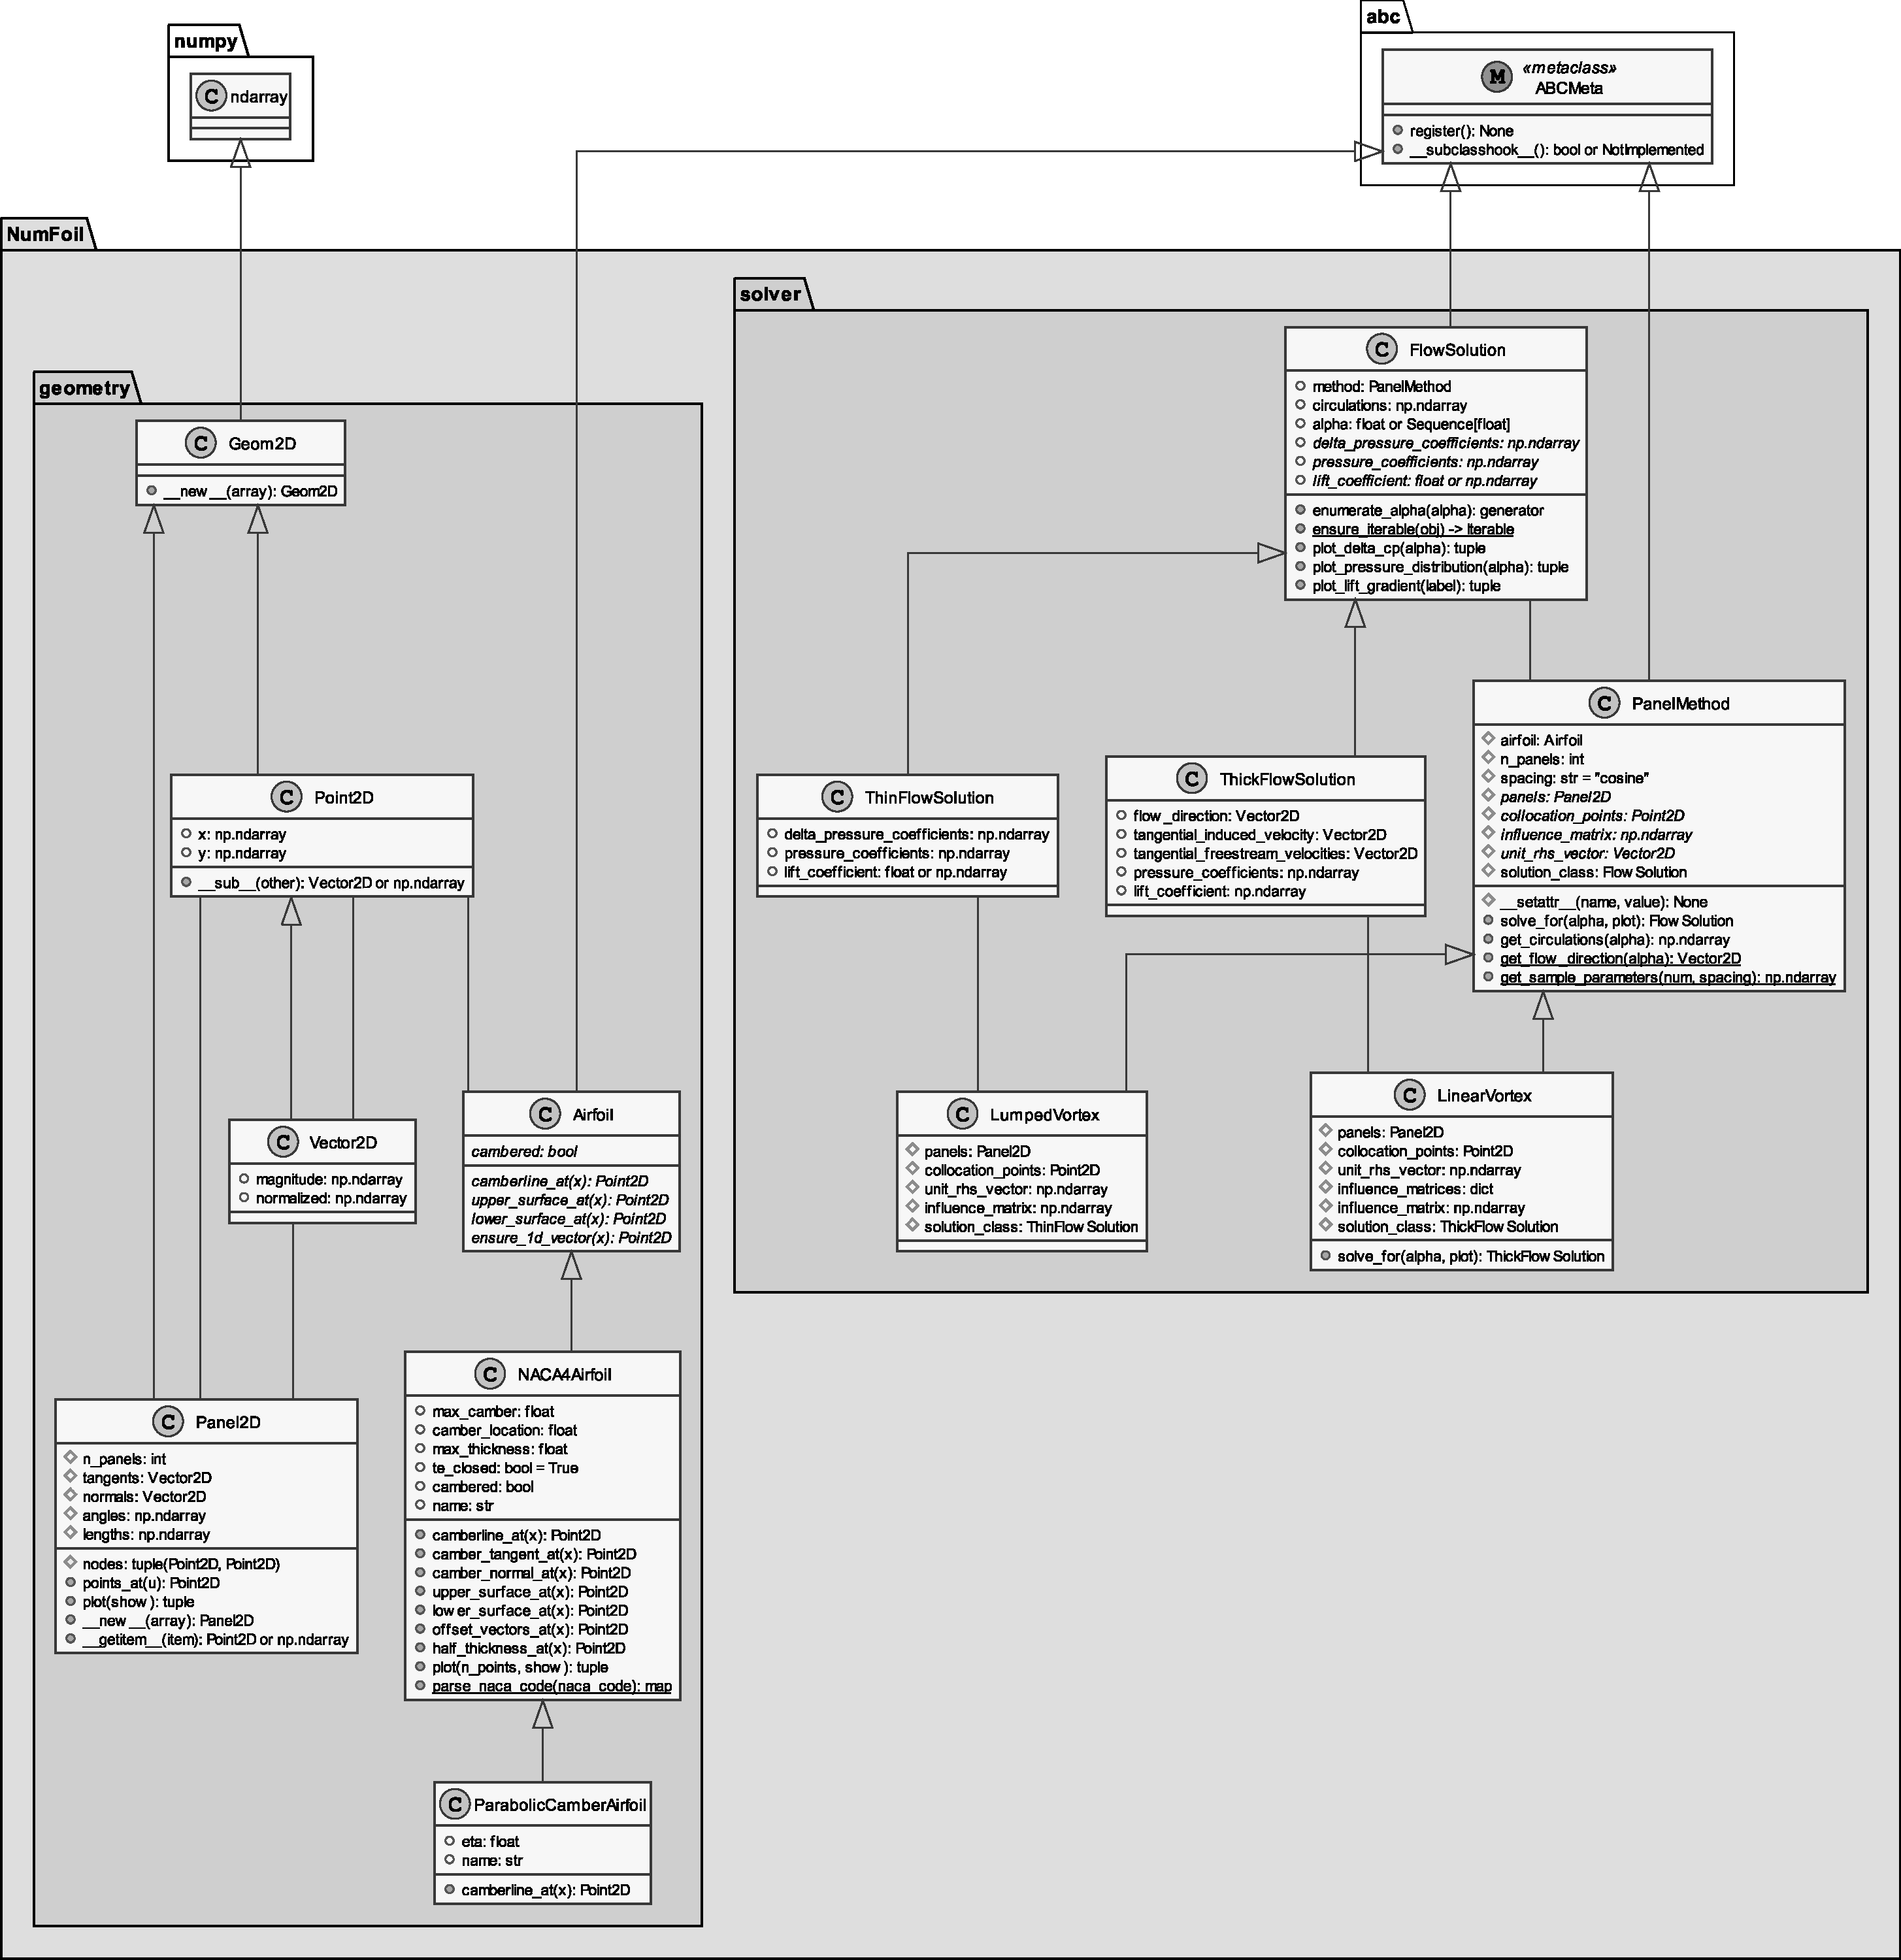
\includegraphics[width=0.85\textwidth]{static/class_diagram.pdf}
    \caption{UML Class Diagram of the \numfoil Package}
\end{figure}

\newpage

\section{NACA 4-Series Airfoil Geometry Class}
\inputminted[firstline=133,lastline=301]{python}{../src/numfoil/geometry/airfoil.py}

\section{Panel Geometry Class}
\inputminted{python}{../src/numfoil/geometry/panel.py}

\section{Abstract Base Panel Method Class}
\inputminted[firstline=321,lastline=512]{python}{../src/numfoil/solver/base.py}

\section{Lumped Vortex Panel Method Class}
\inputminted{python}{../src/numfoil/solver/m_lumped_vortex.py}

\section{Thin Flow Solution Class}
\inputminted[firstline=220,lastline=241]{python}{../src/numfoil/solver/base.py}
